\documentclass{beamer}
\usetheme[pageofpages=of,% String used between the current page and the
                         % total page count.
          bullet=circle,% Use circles instead of squares for bullets.
          titleline=true,% Show a line below the frame title.
          alternativetitlepage=true,% Use the fancy title page.
	  titlepagelogo=logo-circl.pdf,% Logo for the first page.
%          watermark=watermark-polito,% Watermark used in every page.
%          watermarkheight=100px,% Height of the watermark.
%          watermarkheightmult=4,% The watermark image is 4 times bigger
                                % than watermarkheight.
          ]{Torino}

\usepackage[utf8x]{inputenc}
\usepackage{listings}
\usepackage{soul}
\usepackage{siunitx}
\usepackage{booktabs}
\usepackage{pdfpages}
%\lstset{ 
%  backgroundcolor=\color{white},   % choose the background color; you must add \usepackage{color} or \usepackage{xcolor}
%  basicstyle=\footnotesize,        % the size of the fonts that are used for the code
%  breakatwhitespace=false
%}

\usepackage{tikz}
\usetikzlibrary{shapes,snakes,automata,positioning,matrix,fit,arrows,shapes.geometric}


\usepackage[listings]{tcolorbox}
\usepackage{xcolor}
\usepackage{colortbl}
\definecolor{mygreen}{rgb}{0,0.6,0}
\definecolor{mygreen2}{rgb}{0,0.56,0.16}
\definecolor{myred}{rgb}{0.6,0.066,0.066}
\definecolor{redCIRCL}{RGB}{213,43,30}
\definecolor{mygray}{rgb}{0.5,0.5,0.5}
\definecolor{mymauve}{rgb}{0.58,0,0.82}
\definecolor{mygray}{gray}{0.9}
\definecolor{mywhite}{rgb}{1,1,1}
\definecolor{myblack}{rgb}{0,0,0}
\definecolor{mybeige}{HTML}{eeeeee}
%\usepackage{tcolorbox}
\usepackage[listings]{tcolorbox}
\tcbuselibrary{listings}

\lstdefinestyle{code}{ %
  backgroundcolor=\color{mybeige},   % choose the background color; you must add \usepackage{color} or \usepackage{xcolor}; should come as last argument
  basicstyle=\footnotesize\ttfamily,        % the size of the fonts that are used for the code
  breakatwhitespace=false,         % sets if automatic breaks should only happen at whitespace
  breaklines=true,                 % sets automatic line breaking
  captionpos=b,                    % sets the caption-position to bottom
  commentstyle=\color{mygreen},    % comment style
  deletekeywords={...},            % if you want to delete keywords from the given language
  escapeinside={\%*}{*)},          % if you want to add LaTeX within your code
  extendedchars=true,              % lets you use non-ASCII characters; for 8-bits encodings only, does not work with UTF-8
  frame=single,	                   % adds a frame around the code
  keepspaces=true,                 % keeps spaces in text, useful for keeping indentation of code (possibly needs columns=flexible)
  keywordstyle=\color{blue},       % keyword style
%   language=Python,                 % the language of the code
  morekeywords={*,...},           % if you want to add more keywords to the set
  numbers=left,                    % where to put the line-numbers; possible values are (none, left, right)
  numbersep=5pt,                   % how far the line-numbers are from the code
  numberstyle=\tiny\color{myblack}, % the style that is used for the line-numbers
  rulecolor=\color{black},         % if not set, the frame-color may be changed on line-breaks within not-black text (e.g. comments (green here))
  showspaces=false,                % show spaces everywhere adding particular underscores; it overrides 'showstringspaces'
  showstringspaces=false,          % underline spaces within strings only
  showtabs=false,                  % show tabs within strings adding particular underscores
  stepnumber=1,                    % the step between two line-numbers. If it's 1, each line will be numbered
  stringstyle=\color{mymauve},     % string literal style
  tabsize=2,	                   % sets default tabsize to 2 spaces
  title=\lstname                   % show the filename of files included with \lstinputlisting; also try caption instead of title
}
\lstdefinestyle{bash}{ %
  backgroundcolor=\color{black!85},   % choose the background color; you must add \usepackage{color} or \usepackage{xcolor}; should come as last argument
  basicstyle=\footnotesize\color{mywhite},        % the size of the fonts that are used for the code
  breakatwhitespace=false,         % sets if automatic breaks should only happen at whitespace
  breaklines=true,                 % sets automatic line breaking
  captionpos=b,                    % sets the caption-position to bottom
  commentstyle=\color{mygreen},    % comment style
  deletekeywords={...},            % if you want to delete keywords from the given language
  escapeinside={\%*}{*)},          % if you want to add LaTeX within your code
  extendedchars=true,              % lets you use non-ASCII characters; for 8-bits encodings only, does not work with UTF-8
  frame=single	                   % adds a frame around the code
  keepspaces=true,                 % keeps spaces in text, useful for keeping indentation of code (possibly needs columns=flexible)
  keywordstyle=\color{white}\bfseries,       % keyword style
  language=bash,                 % the language of the code
  morekeywords={*,$,git, clone,... },           % if you want to add more keywords to the set
  numbers=left,                    % where to put the line-numbers; possible values are (none, left, right)
  numbersep=5pt,                   % how far the line-numbers are from the code
  numberstyle=\tiny\color{mywhite}, % the style that is used for the line-numbers
  rulecolor=\color{black},         % if not set, the frame-color may be changed on line-breaks within not-black text (e.g. comments (green here))
  showspaces=false,                % show spaces everywhere adding particular underscores; it overrides 'showstringspaces'
  showstringspaces=false,          % underline spaces within strings only
  showtabs=false,                  % show tabs within strings adding particular underscores
  stepnumber=1,                    % the step between two line-numbers. If it's 1, each line will be numbered
  stringstyle=\color{mymauve},     % string literal style
  tabsize=2,	                   % sets default tabsize to 2 spaces
  title=\lstname                   % show the filename of files included with \lstinputlisting; also try caption instead of title
}
\lstdefinestyle{default}{ %
  backgroundcolor=\color{white},   % choose the background color; you must add \usepackage{color} or \usepackage{xcolor}; should come as last argument
  basicstyle=\footnotesize\color{black},        % the size of the fonts that are used for the code
  breakatwhitespace=false,         % sets if automatic breaks should only happen at whitespace
  breaklines=true,                 % sets automatic line breaking
  captionpos=b,                    % sets the caption-position to bottom
  commentstyle=\color{mygreen},    % comment style
  deletekeywords={...},            % if you want to delete keywords from the given language
  escapeinside={\%*}{*)},          % if you want to add LaTeX within your code
  extendedchars=true,              % lets you use non-ASCII characters; for 8-bits encodings only, does not work with UTF-8
  frame=single	                   % adds a frame around the code
  keepspaces=true,                 % keeps spaces in text, useful for keeping indentation of code (possibly needs columns=flexible)
  keywordstyle=\color{white}\bfseries,       % keyword style
  language=bash,                 % the language of the code
  morekeywords={*,$,git, clone,... },           % if you want to add more keywords to the set
  numbers=left,                    % where to put the line-numbers; possible values are (none, left, right)
  numbersep=5pt,                   % how far the line-numbers are from the code
  numberstyle=\tiny\color{black}, % the style that is used for the line-numbers
  rulecolor=\color{black},         % if not set, the frame-color may be changed on line-breaks within not-black text (e.g. comments (green here))
  showspaces=false,                % show spaces everywhere adding particular underscores; it overrides 'showstringspaces'
  showstringspaces=false,          % underline spaces within strings only
  showtabs=false,                  % show tabs within strings adding particular underscores
  stepnumber=1,                    % the step between two line-numbers. If it's 1, each line will be numbered
  stringstyle=\color{mymauve},     % string literal style
  tabsize=2,	                   % sets default tabsize to 2 spaces
  title=\lstname                   % show the filename of files included with \lstinputlisting; also try caption instead of title
}
\lstset{style=code}


% \AtBeginSection[]{
% 	\begin{frame}[fragile]
%   \vfill
%   \centering
%   \begin{beamercolorbox}[sep=8pt,center,shadow=true,rounded=true]{title}
%       {\color{white} \usebeamerfont{title}\insertsectionhead}\par%
%   \end{beamercolorbox}
%   \vfill
%   \end{frame}
% }

\author{\large{Alexandre Dulaunoy}\\ \scriptsize{alexandre.dulaunoy@circl.lu}\\ \large{Jean-Louis Huynen}\\ \scriptsize{jean-louis.huynen@circl.lu}\\ \large{Sami Mokaddem}\\ \scriptsize{sami.mokaddem@circl.lu}\\}
\title{Introduction to pattern matching}
\subtitle{Using Regexes}
\institute{info@circl.lu}
\date{\today}
\begin{document}


\begin{frame}[t,plain]
\titlepage
\end{frame}

\begin{frame}[fragile]
\frametitle{Typical Linux problem}
\begin{lstlisting}
$ cat files.txt
readme.md
document.pdf
image.png
music.mp3
video.mp4
manual.pdf
\end{lstlisting}

    \begin{center}
         \textbf{Objectives}: List only PDF files
    \end{center}
\end{frame}

\begin{frame}[fragile]
\frametitle{\texttt{\$ man grep}}
\begin{lstlisting}
GREP(1)             User Commands               GREP(1)

NAME
    grep, egrep, fgrep, rgrep - print lines that match patterns

SYNOPSIS
    grep [OPTION...] PATTERNS [FILE...]
    grep [OPTION...] -e PATTERNS ... [FILE...]
    grep [OPTION...] -f PATTERN_FILE ... [FILE...]

DESCRIPTION
    grep searches for PATTERNS in each FILE.  PATTERNS is one or more patterns separated  by  newline  characters,  and  grep prints each line that matches a pattern.  Typically PATTERNS should be quoted when grep is used in a shell command.
\end{lstlisting}
\end{frame}

\begin{frame}[fragile]
\frametitle{Using \texttt{grep}}
\begin{lstlisting}
$ cat files.txt | grep 'pdf'
document.pdf
manual.pdf
\end{lstlisting}
\begin{center}
    Easy! However...
\end{center}
\pause
\begin{lstlisting}
$ cat files-2.txt | grep 'pdf'
document.pdf
manual.pdf
homework.pdf.jpg
\end{lstlisting}

\begin{center}
    How can we filter out \texttt{homework.pdf.jpg}?
\end{center}
\end{frame}

\begin{frame}[fragile]
\frametitle{Using \texttt{grep}}
\begin{lstlisting}
$ cat files-2.txt | grep 'pdf' | grep -v 'jpg'
document.pdf
manual.pdf
\end{lstlisting}
\begin{center}
    \texttt{-v} allows us to perform an in\textbf{V}ert match
\end{center}
    \begin{center}
    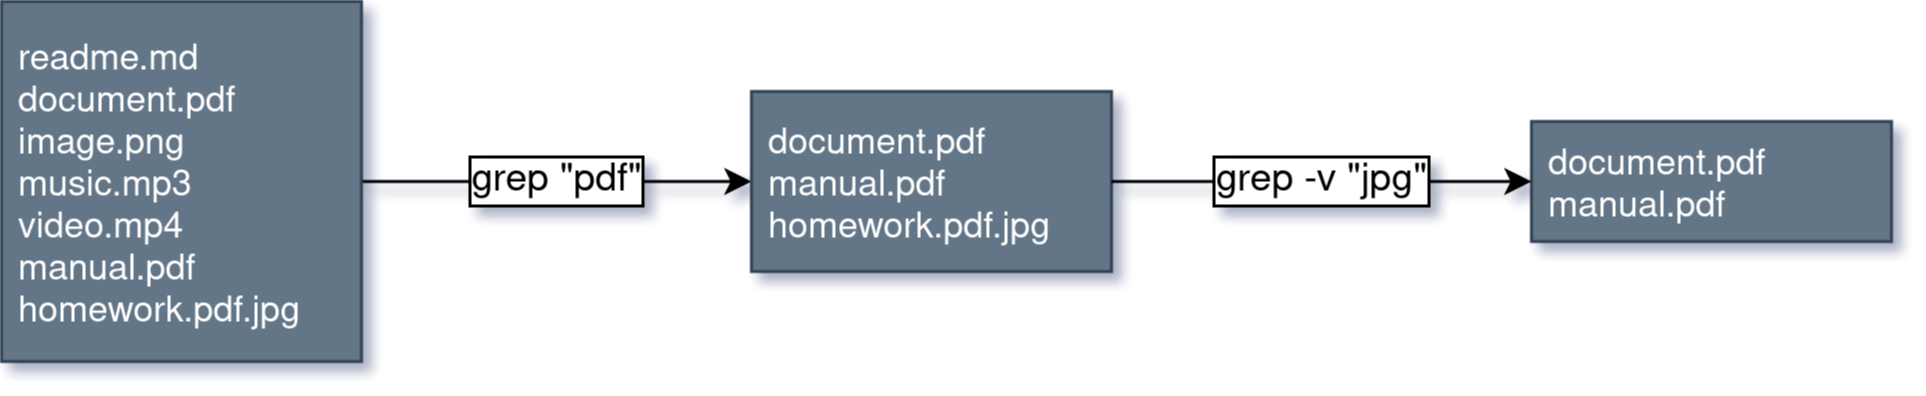
\includegraphics[width=1.0\textwidth]{pics/linux_pipe_diagram.png}
    \end{center}
\end{frame}


\begin{frame}[fragile]
\frametitle{Using \texttt{grep}}
\begin{lstlisting}
$ cat files-3.txt | grep 'pdf' | grep -v 'jpg'
document.pdf
manual.pdf
adobe_pdf_reader.exe
i_hate_pdf.mp3
this.is.a.weird.pdf.filename.zip
filename with spaces are evil.pdf
\end{lstlisting}
\begin{center}
    Using invert match is not going to scale...
\end{center}
\end{frame}

\begin{frame}[fragile]
\frametitle{Other commonly encountered problems}
    \begin{itemize}
        \item Matching valid email addresses
        \item Matching valid IBAN number
        \item Matching valid IPv4 addresses
    \end{itemize}
    \vspace{1em}
    \begin{center}
        $\rightarrow$ Regular Expressions (\textbf{Regex}) to the rescue
    \end{center}
\end{frame}

\begin{frame}[fragile]
    \frametitle{Regular Expression}
    \begin{center}
        A \textbf{regular expression} (shortened as \textbf{regex} or \textbf{regexp}) is a sequence of characters that specifies a search pattern in text.
    \end{center}
    \begin{center}
        \textbf{Regexes} are extremely useful in extracting information from text.
    \end{center}
\end{frame}

\begin{frame}[fragile]
    \frametitle{Regular Expression Basics}
    \begin{itemize}
        \item What ?
        \begin{itemize}
            \item Literal characters: \texttt{abc}
            \item Quantifiers: \texttt{ab+c}
            \item Operator OR: \texttt{(abc|cba)}
            \item Bracket expressions: \texttt{[a-z]}
            \item Meta sequences: \texttt{\textbackslash S}
            \item Capture group: \texttt{(abc)}
            \item Anchors: \texttt{\textasciicircum abc\$}
        \end{itemize}
        \item New skill ?
        \vspace{1em}
        \begin{verbatim}/ <([a-z]+)(>(.*)<\/\1>|\s+\/>) /\end{verbatim}
    \end{itemize}
\end{frame}

\begin{frame}[fragile]
    \frametitle{Regular Expression Basics: Literal characters}
    \begin{center}
        Letters and digits from the ASCII character set match their respective value
    \end{center}
    \begin{center}
    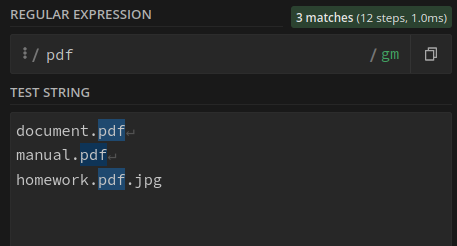
\includegraphics[width=1.0\textwidth]{pics/regex/regex1.png}
    \end{center}
\end{frame}

\begin{frame}[fragile]
    \frametitle{Regular Expression Basics: The Dot}
    \begin{center}
        \texttt{\Large .} is a \textit{joker} or \textit{wildcard} that can match any single character
    \end{center}
    \begin{center}
    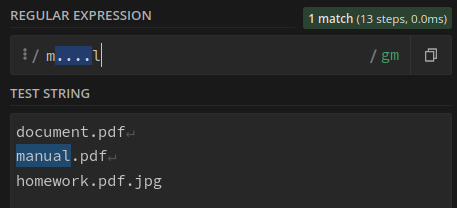
\includegraphics[width=1.0\textwidth]{pics/regex/regex2.png}
    \end{center}
\end{frame}

\begin{frame}[fragile]
    \frametitle{Regular Expression Basics: The Period}
    \begin{center}
        The period character \texttt{\Large .} can be matched using the escape character \texttt{\textbackslash .}
    \end{center}
    \begin{center}
    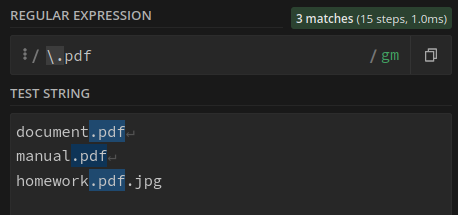
\includegraphics[width=1.0\textwidth]{pics/regex/regex3.png}
    \end{center}
\end{frame}

\begin{frame}[fragile]
    \frametitle{Regular Expression Basics: OR Operator}
    \begin{center}
        The \texttt{\Large ( | )} structure can be used as a logical operator to match one sequence or the other
    \end{center}
    \begin{center}
        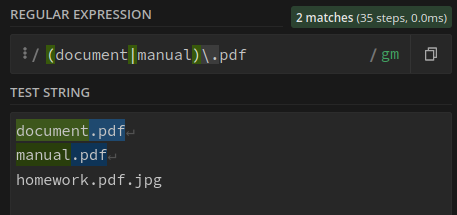
\includegraphics[width=1.0\textwidth]{pics/regex/regex16.png}
    \end{center}
\end{frame}

\begin{frame}[fragile]
    \frametitle{Regular Expression Basics: Bracket Expression (1)}
    \begin{center}
        The \texttt{\Large [ \;  ]} structure can be used to specifiy a set of characters that can match
    \end{center}
    \begin{center}
        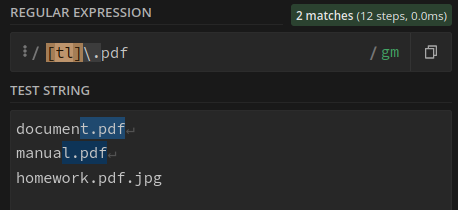
\includegraphics[width=1.0\textwidth]{pics/regex/regex4.png}
    \end{center}
\end{frame}

\begin{frame}[fragile]
    \frametitle{Regular Expression Basics: Bracket Expression (2)}
    \begin{center}
        The \texttt{\Large [\textasciicircum \; ]} structure can be used to exclude a specific set of characters
    \end{center}
    \begin{center}
    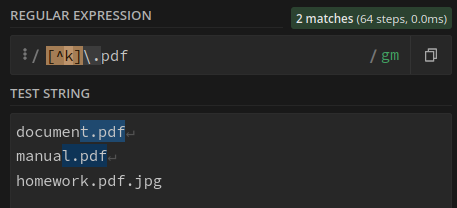
\includegraphics[width=1.0\textwidth]{pics/regex/regex5.png}
    \end{center}
\end{frame}

\begin{frame}[fragile]
    \frametitle{Regular Expression Basics: Bracket Expression (3)}
    \begin{center}
        The \texttt{\Large [ \thinspace - \thinspace ]} structure can be used to specifiy a range of sequential characters
    \end{center}
    \begin{center}
    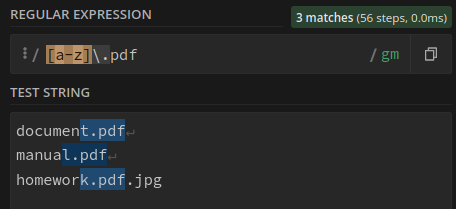
\includegraphics[width=1.0\textwidth]{pics/regex/regex6.png}
    \end{center}
\end{frame}

% \colorbox{blue!50}{\makebox[1em]{\strut}
% \colorbox{red!90}{\makebox[1em]{\strut}
% \colorbox{blue!50}{\makebox{\strut one}}
% \colorbox{red!90}{\makebox{\strut one}}
\begin{frame}[fragile]
    \frametitle{Regular Expression Basics: Meta Sequences (1)}
    \begin{itemize}
        \item \begin{verbatim}/ . /\end{verbatim}
        \begin{itemize}
            \item Any single character
        \end{itemize}
        \item \begin{verbatim}/ \w /\end{verbatim}
        \begin{itemize}
            \item Any word character
            \item \begin{verbatim}/ [a-zA-Z0-9_] /\end{verbatim}
            \item \textbf{Match}: \texttt{\colorbox{blue!50}{\makebox[1em]{\strut any}}\colorbox{red!90}{\makebox[1em]{\strut}}\colorbox{blue!50}{\makebox{\strut non-whitespace}}\colorbox{red!90}{\makebox[1em]{\strut}}\colorbox{blue!50}{\makebox{\strut character}}\colorbox{red!90}{\makebox[1em]{\strut}}\colorbox{red!90}{\makebox{\strut \$!-:;}}}
        \end{itemize}
        \item \begin{verbatim}/ \W /\end{verbatim}
        \begin{itemize}
            \item Any non-word character
            \item \begin{verbatim}/ [^a-zA-Z0-9_] /\end{verbatim}
            \item \textbf{Match}: \texttt{\colorbox{red!90}{\makebox[1em]{\strut any}}\colorbox{blue!50}{\makebox[1em]{\strut}}\colorbox{red!90}{\makebox{\strut whitespace}}\colorbox{blue!50}{\makebox[1em]{\strut}}\colorbox{red!90}{\makebox{\strut character}}\colorbox{blue!50}{\makebox[1em]{\strut}}\colorbox{blue!50}{\makebox{\strut \$!-:;}}}
        \end{itemize}
    \end{itemize}
\end{frame}

\begin{frame}[fragile]
    \frametitle{Regular Expression Basics: Meta Sequences (2)}
    \begin{itemize}
        \item \begin{verbatim}/ \d /\end{verbatim}
        \begin{itemize}
            \item Any digit
            \item \textbf{Match}: \texttt{\colorbox{red!90}{\makebox{\strut one: }}\colorbox{blue!50}{\makebox[1em]{\strut 1}}\colorbox{red!90}{\makebox{\strut, two: }}\colorbox{blue!50}{\makebox[1em]{\strut 2}}\colorbox{red!90}{\makebox{\strut ;}}}
        \end{itemize}
        \item \begin{verbatim}/ \s /\end{verbatim}
        \begin{itemize}
            \item Any whitespace character
            \item \textbf{Match}: \texttt{\colorbox{red!90}{\makebox[1em]{\strut any}}\colorbox{blue!50}{\makebox[1em]{\strut}}\colorbox{red!90}{\makebox{\strut whitespace}}\colorbox{blue!50}{\makebox[1em]{\strut}}\colorbox{red!90}{\makebox{\strut character}}\colorbox{blue!50}{\makebox[1em]{\strut}}\colorbox{red!90}{\makebox{\strut \$!-:;}}}
        \end{itemize}
        \item \begin{verbatim}/ \S /\end{verbatim}
        \begin{itemize}
            \item Any non-whitespace character
            \item \textbf{Match}: \texttt{\colorbox{blue!50}{\makebox[1em]{\strut any}}\colorbox{red!90}{\makebox[1em]{\strut}}\colorbox{blue!50}{\makebox{\strut non-whitespace}}\colorbox{red!90}{\makebox[1em]{\strut}}\colorbox{blue!50}{\makebox{\strut character}}\colorbox{red!90}{\makebox[1em]{\strut}}\colorbox{blue!50}{\makebox{\strut \$!-:;}}}
        \end{itemize}
    \end{itemize}
\end{frame}

\begin{frame}[fragile]
    \frametitle{Regular Expression Basics: Reading Exercises (1)}
    \begin{enumerate}
        \item \begin{verbatim}/ facebo.k /\end{verbatim}
        \pause
        \begin{itemize}
            \item \textbf{Match}: \texttt{facebook}, \texttt{faceboak}, \texttt{facebo\&k}
        \end{itemize}
        \item \begin{verbatim}/ 4\.2 /\end{verbatim}
        \pause
        \begin{itemize}
            \item \textbf{Match}: \texttt{4.2}
            \item \textbf{Match}: \texttt{Nice number: 4.2}
        \end{itemize}
        \item \begin{verbatim}/ drink (beer|wine) ! /\end{verbatim}
        \pause
        \begin{itemize}
            \item \textbf{Match}: \texttt{I drink beer !}
            \item \textbf{Match}: \texttt{I drink wine !}
        \end{itemize}
        \item \begin{verbatim}/ [e-h] /\end{verbatim}
        \pause
        \begin{itemize}
            \item \textbf{Match}: \texttt{fefe}, \texttt{hehe}
            \item \textbf{No match}: \st{\texttt{haha}}
        \end{itemize}
    \end{enumerate}
\end{frame}

\begin{frame}[fragile]
    \frametitle{Regular Expression Basics: Writing Exercises (1)}
    \begin{enumerate}
        \item \textbf{Match}: \textit{red\_light}, \textit{green\_light} and \textit{~!=\_light}
        \pause
        \begin{itemize}
            \item[] \begin{verbatim}/ _light /\end{verbatim}
        \end{itemize}
        \item \textbf{Match}: \textit{red\_light} and \textit{green\_light} \textbf{but not} \textit{white\_light}
        \pause
        \begin{itemize}
            \item[] \begin{verbatim}/ (red|green)_light /\end{verbatim}
        \end{itemize}
        \item \textbf{Match}: \textit{*\_light} where \texttt{*} is any digit
        \pause
        \begin{itemize}
            \item[] \begin{verbatim}/ [0-9]_light /\end{verbatim}
        \end{itemize}
        \item \textbf{Match}: \textit{?\_light} where \texttt{?} is 4-letters color name
        \pause
        \begin{itemize}
            \item[] \begin{verbatim}/ [a-z][a-z][a-z][a-z]_light /\end{verbatim}
        \end{itemize}
        \pause
    \end{enumerate}
    \vspace*{1em}
    \textbf{Question}: \textit{?\_light} where \texttt{?} is any color between 3 and 6 letters
    \begin{center}
        We need a way to express occurences... Introducing \textbf{quantifiers}
    \end{center}
\end{frame}

\begin{frame}[fragile]
    \frametitle{Regular Expression Basics: Quantifiers (1)}
    \begin{center}
        The \texttt{*} control character can be used to describe \textbf{zero or more} occurences
    \end{center}
    \begin{center}
    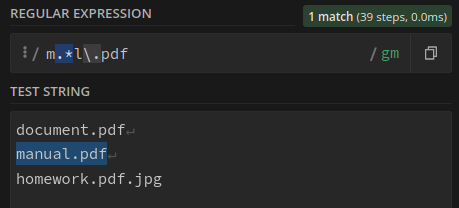
\includegraphics[width=1.0\textwidth]{pics/regex/regex7.png}
    \end{center}
\end{frame}

\begin{frame}[fragile]
    \frametitle{Regular Expression Basics: Quantifiers (2)}
    \begin{center}
        The \texttt{+} control character can be used to describe \textbf{one or more} occurences
    \end{center}
    \begin{center}
    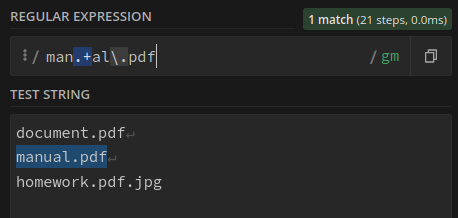
\includegraphics[width=1.0\textwidth]{pics/regex/regex9.png}
    \end{center}
\end{frame}

\begin{frame}[fragile]
    \frametitle{Regular Expression Basics: Quantifiers (3)}
    \begin{itemize}
        \item \begin{verbatim}/ a? /\end{verbatim}
        \begin{itemize}
            \item Match 0 or one \texttt{a} character
        \end{itemize}
        \item \begin{verbatim}/ a{3} /\end{verbatim}
        \begin{itemize}
            \item Match exactly 3 \texttt{a} character
        \end{itemize}
        \item \begin{verbatim}/ a{3,} /\end{verbatim}
        \begin{itemize}
            \item Match 3 or more \texttt{a} character
        \end{itemize}
        \item \begin{verbatim}/ a{3,6} /\end{verbatim}
        \begin{itemize}
            \item Match between 3 and 6 \texttt{a} character
        \end{itemize}
    \end{itemize}
\end{frame}

\begin{frame}[fragile]
    \frametitle{Regular Expression Basics: Reading Exercises (2)}
    \begin{enumerate}
        \item \begin{verbatim}/ colou?r /\end{verbatim}
        \pause
        \begin{itemize}
            \item \textbf{Match}: \texttt{colour} and \texttt{color}
        \end{itemize}
        \item \begin{verbatim}/ go*gle /\end{verbatim}
        \pause
        \begin{itemize}
            \item \textbf{Match}: \texttt{gogle}, \texttt{gooooogle}, \texttt{ggle}, ...
        \end{itemize}
        \item \begin{verbatim}/ waz+up /\end{verbatim}
        \pause
        \begin{itemize}
            \item \textbf{Match}: \texttt{wazup}, \texttt{wazzzzzup}, ...
        \end{itemize}
        \item \begin{verbatim}/ +352[0-9]{6,8} /\end{verbatim}
        \pause
        \begin{itemize}
            \item \textbf{Match}: \texttt{+352791648}, \texttt{+35226791349}
        \end{itemize}
    \end{enumerate}
\end{frame}

\begin{frame}[fragile]
    \frametitle{Regular Expression Basics: Writing Exercises (2)}
    \begin{enumerate}
        \item \textbf{Match}: The time (16:42, 03:59)
        \pause
        \begin{itemize}
            \item[] \begin{verbatim}/ [0-9][0-9]:[0-9][0-9] /\end{verbatim}
            \item[] (not perfect but good enough for the exercise)
        \end{itemize}
        \item \textbf{Match}: Luxembourg postal code (L-4253, L-1110)
        \pause
        \begin{itemize}
            \item[] \begin{verbatim}/ L-[0-9]{4} /\end{verbatim}
        \end{itemize}
        \item \textbf{Match}: \textit{*\_light} where \texttt{*} is any color?
        \pause
        \begin{itemize}
            \item[] \begin{verbatim}/ [a-z]+_light /\end{verbatim}
        \end{itemize}
        \item \textbf{Match}: any hexadecimnal color (\#ff0000, \#f7f8f9)
        \pause
        \begin{itemize}
            \item[] \begin{verbatim}/ #[a-f0-9]{6} /\end{verbatim}
        \end{itemize}
    \end{enumerate}
\end{frame}

\begin{frame}[fragile]
    \frametitle{Regular Expressions: Final question}
    \begin{center}
        What does these regexes do?
    \end{center}
    \vspace{1em}
    \begin{enumerate}
        \item \begin{verbatim}/ ([12]\d{3}-(0[1-9]|1[0-2])-(0[1-9]|[12]\d|3[01])) /\end{verbatim}
        \vspace{1em}
        \item \begin{verbatim}/ <([a-z]+)(>(.*)<\/\1>|\s+\/>) /\end{verbatim}
        \begin{itemize}
            \item \texttt{\textbackslash 1} is used to reference the first capturing group
            \item First capturing group is \texttt{([a-z]+)}
        \end{itemize}
    \end{enumerate}
\end{frame}

\begin{frame}[fragile]
    \frametitle{Regexes: Going further}
    \begin{itemize}
        \item \textbf{\textasciicircum} and \textbf{\$} anchors
        \item Capture \textbf{groups}
        \item \textbf{Greedy} and \textbf{Lazy} quantifiers
        \item \textbf{Possessive} quantifier
    \end{itemize}
\end{frame}

% grep -ir disney | wc
% grep -ir 'disney' | egrep -i '[a-zA-Z0-9_\-\+\.]+@\w+(\.\w+)+:\S+'
% egrep -inr 'disney(\+)?((_\s)?(plus))?' | egrep -i '[a-zA-Z0-9_\-\+\.]+@\w+(\.\w+)+:\S+'
% egrep -inr 'disney(\+)?((_\s)?(plus))?' | egrep -i '(hotmail|live|outlook|gmail|yahoo)' | egrep -i '[a-zA-Z0-9_\-\+\.]+@\w+(\.\w+)+:\S+'
% egrep -inr 'disney(\+)?((_\s)?(plus))?' | egrep -i '(hotmail|live|outlook|gmail|yahoo)' | egrep -i '[a-zA-Z0-9_\-\+\.]+@\w+(\.\w+)+:\S+' | cut -d ':' -f1 - | sort | uniq
% egrep -inr 'disney(\+)?((_\s)?(plus))?' | egrep -i '(hotmail|live|outlook|gmail|yahoo)' | egrep -i '[a-zA-Z0-9_\-\+\.]+@\w+(\.\w+)+:\S+' | cut -d ':' -f1 - | cut --d ' ' -f1
% egrep -inr '(disney|psn)' | egrep -i '(hotmail|live|outlook|gmail|yahoo)' | egrep -i '[a-zA-Z0-9_\-\+\.]+@\w+(\.\w+)+:\S+' | cut -d ':' -f1 - | cut --d ' ' -f1
% egrep -hiro '[a-zA-Z0-9_\-\+\.]+@\w+(\.\w+)+:\S+' | cut -d ':' -f2 | sort | uniq -c | sort

\begin{frame}
    \vfill
    \centering
    \LARGE Linux commands and Regexes
    \vfill
\end{frame}

\begin{frame}[fragile]
    \frametitle{Linux commands and Regexes}
    You have a small subset of a files crawled on Pastebin
\begin{lstlisting}
$ du -hd1
158M    .
$ ls | wc
11875   11875  106875
\end{lstlisting}
\end{frame}

\begin{frame}[fragile]
    \frametitle{Linux commands and Regexes}
    Let's list the number of files that have the \texttt{disney} keyword
\begin{lstlisting}
$ grep -irl disney | wc
88      88     792
\end{lstlisting}

    Let's filter on common email providers
\begin{lstlisting}
$ egrep -ir 'disney'
    | egrep -i '(hotmail|live|outlook|gmail|yahoo)'
    | wc
52  122772 1566533
\end{lstlisting}
\end{frame}

\begin{frame}[fragile]
    \frametitle{Linux commands and Regexes}
    Let's filter on the \texttt{email:password} pattern
\begin{lstlisting}
$ egrep -ir 'disney'
    | egrep -i '(hotmail|live|outlook|gmail|yahoo)'
    | egrep -i '[a-zA-Z0-9_\-\+\.]+@\w+(\.\w+)+:\S+'
    | wc
13     902   21758
\end{lstlisting}

    Let's extract all credentials and only the credentials
\begin{lstlisting}
$ egrep -ir 'disney'
    | egrep -i '(hotmail|live|outlook|gmail|yahoo)'
    | egrep -io '[a-zA-Z0-9_\-\+\.]+@\w+(\.\w+)+:\S+'
    | wc
13      13     438
\end{lstlisting}
\end{frame}

\begin{frame}[fragile]
    \frametitle{Linux commands and Regexes}
    Let's search for other type of accounts
\begin{lstlisting}
$ egrep -ir 'psn'
    | egrep -i '(hotmail|live|outlook|gmail|yahoo)'
    | egrep -i '[a-zA-Z0-9_\-\+\.]+@\w+(\.\w+)+:\S+'
    | wc
2     124     583
\end{lstlisting}
\end{frame}


\begin{frame}[fragile]
\frametitle{Fun with Regular Expressions}
\texttt{https://regexcrossword.com/}
\begin{center}
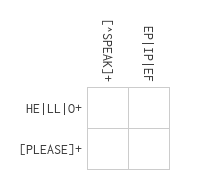
\includegraphics[width=0.4\textwidth]{pics/regex/crossword1.png}
\end{center}
\end{frame}

\begin{frame}[fragile]
\frametitle{Fun with Regular Expressions}
\texttt{https://regexcrossword.com/}
\begin{center}
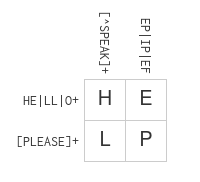
\includegraphics[width=0.4\textwidth]{pics/regex/crossword2.png}
\end{center}
\end{frame}

\begin{frame}[fragile]
\frametitle{Fun with Regular Expressions}
\texttt{https://regexcrossword.com/}
\begin{center}
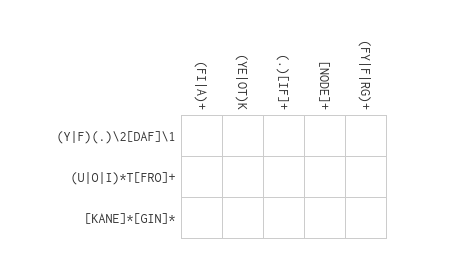
\includegraphics[width=0.8\textwidth]{pics/crosswords}
\end{center}
\end{frame}

\begin{frame}[fragile]
\frametitle{Fun with Regular Expressions}
\texttt{https://regexcrossword.com/}
\begin{center}
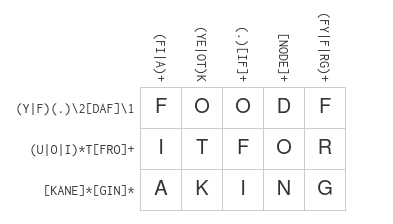
\includegraphics[width=0.8\textwidth]{pics/crosswords-solved.png}
\end{center}
\end{frame}

\begin{frame}[fragile]
    \frametitle{Simple CTF challenge with regular expressions}
    \begin{itemize}
        \item Hidden 4 flags in the dump
        \item They have the following pattern
        \begin{itemize}
            \item \texttt{flag} letters in any order
            \item \texttt{\_} The underscore character
            \item 2 upper case character
            \item at least one special character from the list \texttt{\textbf{@}} , \texttt{\textbf{\&}}, \texttt{\textbf{:}}
            \item 2 lower case character
        \end{itemize}
        \item Example: \texttt{falg\_AA\&:bb}
    \end{itemize}
\end{frame}

\begin{frame}[fragile]
    \frametitle{Simple CTF challenge with regular expressions}
    SHA1 Sum of the flags
    % solution: [flag]{4}_[A-Z]{2}[@&:]+[a-z]{2}
\begin{lstlisting}
$ echo 'falg_AA&:bb' | md5sum
ee9326ee21572fe4bba8e686a7ba6e5e
\end{lstlisting}
    \begin{tabular}{ lr } 
        \texttt{falg\_AA\&:bb} & \texttt{ee9326ee21572fe4bba8e686a7ba6e5e} \\
        \texttt{?} & \texttt{53923b8f8490072107b3e8bb614749ce} \\
        \texttt{?} & \texttt{429698c6d1742f02212ae89d3696577d} \\
        \texttt{?} & \texttt{40178e8ef4264385fb7194176faf2318} \\
       \end{tabular}
\end{frame}

\begin{frame}
    \vfill
    \centering
    \Huge Annex
    \vfill
\end{frame}

\begin{frame}[fragile]
    \frametitle{Regular Expressions: Tag matching (1)}
    Create a Regex that validates the following tags:
\begin{lstlisting}
namespace:predicate
namespace:predicate="value"
name_space:pred_icate="value"
namespace:predicate="qwert _+$- yuiop"
namespace:predicate="qwert=:yuiop"
\end{lstlisting}
    But not these:
\begin{lstlisting}
tag
name space:pred icate="value"
name-space:predicate="value"
namespace:predicate="qwert"yuiop"
\end{lstlisting}
\end{frame}

\begin{frame}[fragile]
    \frametitle{Regular Expressions: Tag matching (2)}
    A valid tag is composed of 2 or 3 parts
    \begin{center}
        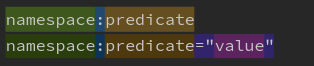
\includegraphics[width=0.66\textwidth]{pics/regex/regex_intro.png}
    \end{center}
    \begin{enumerate}
        \item The \texttt{namespace}
        \item The \texttt{predicate}
        \item The optional \texttt{value}
    \end{enumerate}
\end{frame}

\begin{frame}[fragile]
    \frametitle{Regular Expressions: Tag matching (3)}
    \begin{center}
        Tag validator
    \end{center}
    {
        \Large
        \begin{verbatim}/ ^([\w]+):([\w]+)(="([^\n"]+)")?$ /\end{verbatim}
    }
\end{frame}

\begin{frame}[fragile]
    \frametitle{Regular Expressions: Tag matching (4)}
    \begin{center}
        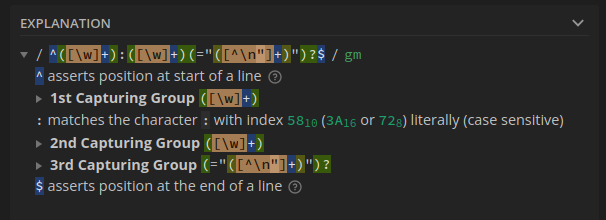
\includegraphics[width=1.0\textwidth]{pics/regex/regex_tag1.png}
    \end{center}
\end{frame}

\begin{frame}[fragile]
    \frametitle{Regular Expressions: Tag matching (5)}
    \begin{center}
        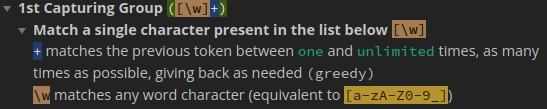
\includegraphics[width=1.0\textwidth]{pics/regex/regex_tag2.png}
    \end{center}
\end{frame}

\begin{frame}[fragile]
    \frametitle{Regular Expressions: Tag matching (5)}
    \begin{center}
        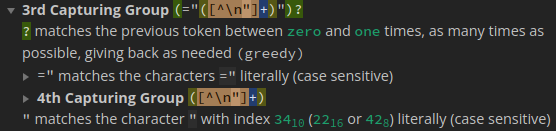
\includegraphics[width=1.0\textwidth]{pics/regex/regex_tag3.png}
    \end{center}
    \begin{center}
        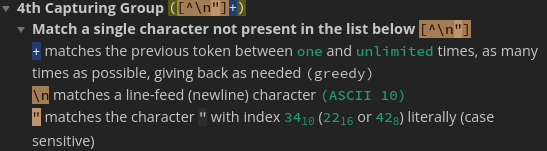
\includegraphics[width=1.0\textwidth]{pics/regex/regex_tag4.png}
    \end{center}
\end{frame}

\end{document}

